\documentclass{scrartcl}

\usepackage{amssymb}
\usepackage{amsmath}
\usepackage{tikz}
\usepackage{xcolor}						%for fill=lightgray
\definecolor{lightgray}{gray}{0.9}		%can adjust last parameter

%Brunnermeier, M. \& Pedersen, L. (2009). ``Market Liquidity and Funding Liquidity.'' The Review of Financial Studies 22(6), pp. 2201-38 -- p. 2204, fig. 2

\begin{document}
	
	%\begin{figure}
	%	\centering
	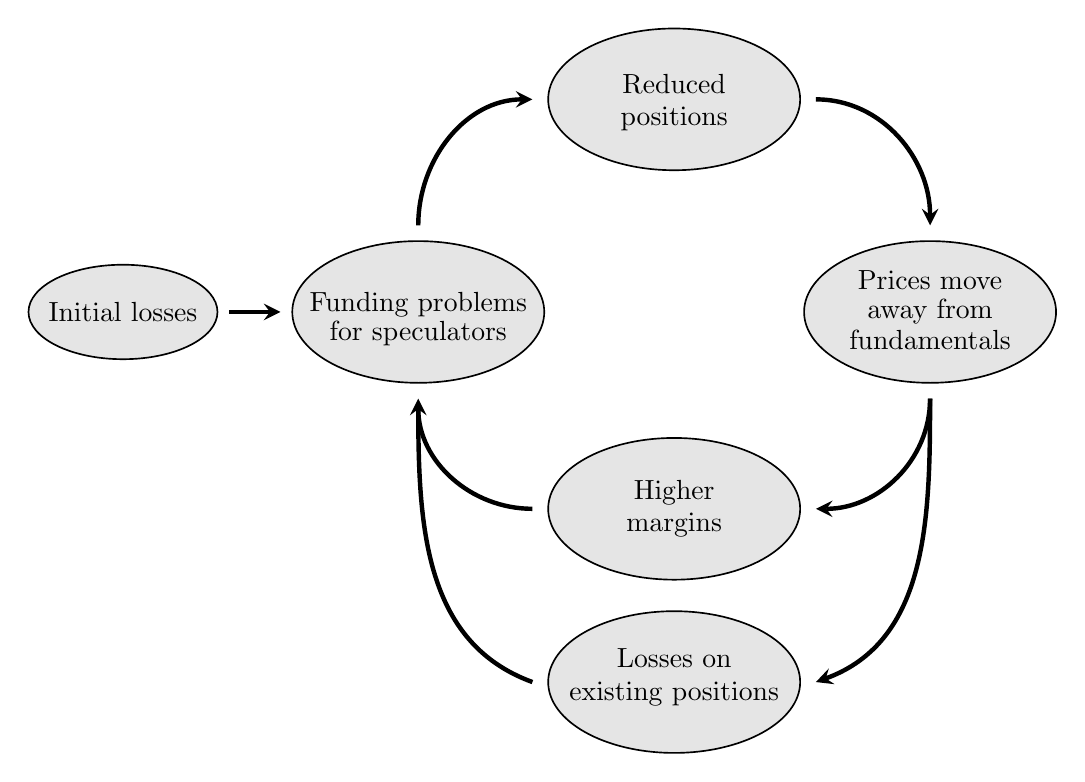
\begin{tikzpicture}
	%ellipses
	\draw[semithick,fill=lightgray] (-7,2.5) circle [x radius=1.2cm, y radius=6mm];
		\node at (-7,2.5)  {Initial losses};
	
	\draw[semithick,fill=lightgray] (0,5.2) circle [x radius=1.6cm, y radius=9mm];
		\node at (0,5.40) {Reduced};
		\node at (0,4.95) {positions};
	
	\draw[semithick,fill=lightgray] (-3.25,2.5) circle [x radius=1.6cm, y radius=9mm];
		\node at (-3.25,2.6)  {Funding problems};
		\node at (-3.25,2.22) {for speculators};
	
	\draw[semithick,fill=lightgray] (0,0) circle [x radius=1.6cm, y radius=9mm];
		\node at (0, 0.2) {Higher};
		\node at (0,-0.2) {margins};
	
	\draw[semithick,fill=lightgray] (3.25,2.5) circle [x radius=1.6cm, y radius=9mm];
		\node at (3.25,2.9)  {Prices move};
		\node at (3.25,2.5)  {away from};
		\node at (3.25,2.15) {fundamentals};
	
	\draw[semithick,fill=lightgray] (0,-2.2) circle [x radius=1.6cm, y radius=9mm];
		\node at (0,-1.90) {Losses on};
		\node at (0,-2.35) {existing positions};
	
	%arrows
	\draw[->,>=stealth,ultra thick] (-5.65,2.5)--(-5,2.5);						%initial--funding
	\draw[->,>=stealth,ultra thick] (-3.25,3.6) to[out=90,in=180] (-1.8,5.2);	%funding--reduced
	\draw[->,>=stealth,ultra thick] (1.8,5.2) to[out=0,in=90] (3.25,3.6);		%reduced--prices
	\draw[->,>=stealth,ultra thick] (3.25,1.4) to[out=270,in=0] (1.8,0);		%prices--higher
	\draw[->,>=stealth,ultra thick] (-1.8,0) to[out=180,in=270] (-3.25,1.4);	%higher-funding
	%
	\draw[->,>=stealth,ultra thick] (3.25,1.4) to[out=270,in=20] (1.8,-2.2);	%prices--losses
	\draw[ultra thick] (-1.8,-2.2) to[out=160,in=270] (-3.25,1.3);				%losses-funding
	\end{tikzpicture}
	%	\caption{Liquidity spirals -- the loss spiral and margin/haricut spiral}
	%\end{figure}
	
\end{document}